%\chapter{Project Progression}
\section{Iterations}
\subsection{Iteration 1 - Prototyping}
  At the beginning, there was a lot of new stuff we had to grow familiar with. We were planning to use a new programming language, new web framework, new database software, new process model, new library for interaction with KNX, which was also new to one of us, and to top it all off, we weren't exactly sure what the product would look like in the end. So, the goal of this iteration was to get familiar with all the used technologies and to establish a direction for user interaction design which we could build on in the later iterations.

  Gabriel's task was to get familiar with calimero as well as to establish a basic widget design using HTML, JavaScript and CSS. He quickly decided to use the JQuery JavaScript framework due to its potency and ease of use. He went on to create basic lamp and temperature widgets, which were fully controllable on the UI side and didn't change a lot until project end. The lamp widget even had working KNX support in the end.

  Meanwhile, Alexander used Lift templates and Scala to build the site structure. He also set up the database and added the first tables for Rooms and Widgets. He also integrated Lift's default user management, which didn't interact with the rest of the site in any way at that time.

  At the end, we had an ugly, but partially working, site in place. While it was still very uncomfortable to use or look at, the most basic functionality was there.
  \begin{figure}[h]
  \centering
  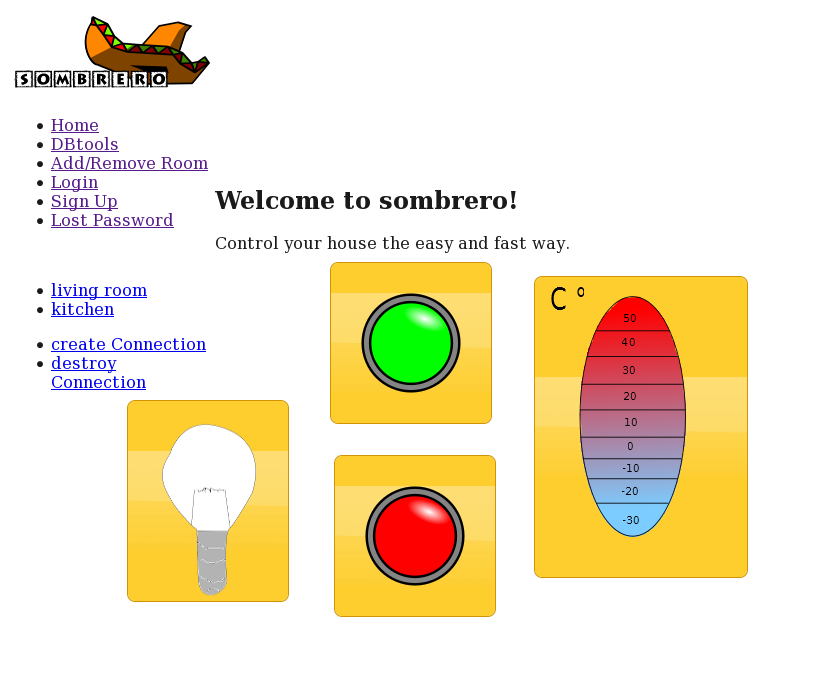
\includegraphics[width=0.80\linewidth]{iteration1.png}
  \caption{the humble beginnings}
  \label{fig:iterations1}
  \end{figure}


\clearpage
\subsection{Iteration 2 - Working}
  With a working prototype to start with, we needed to add all the core functionality which was required for the application to be useful in everyday life.

  The main points were:
  \begin{itemize}
    \item Room management had to be simplified.
    \item User functionality had to be integrated into the site concept.
    \item Widget management was needed.
    \item Image uploading functionality for rooms had to be implemented.
    \item We needed some utility widgets, mainly links between rooms, a toolbox for administrators and a favorite bar for users.
    \item KNX support had to be extended to non-Lamp widgets.
    \item Router discovery for establishing a connection to the KNX network had to be implemented.
    \item We \emph{desperately} needed a more appealing design.
  \end{itemize}

  Building on their experience, Gabriel took care of design and layout, improving the widget concept and expanding KNX support while Alexander managed the database and management functionality and implemented KNX utility features.

  At the end of this iteration, the core functionality was there. The site was still incoherent and parts of the code were a mess, but most of it \emph{worked} and it would have probably been usable by someone brave enough.

  \begin{figure}[h]
  \centering
  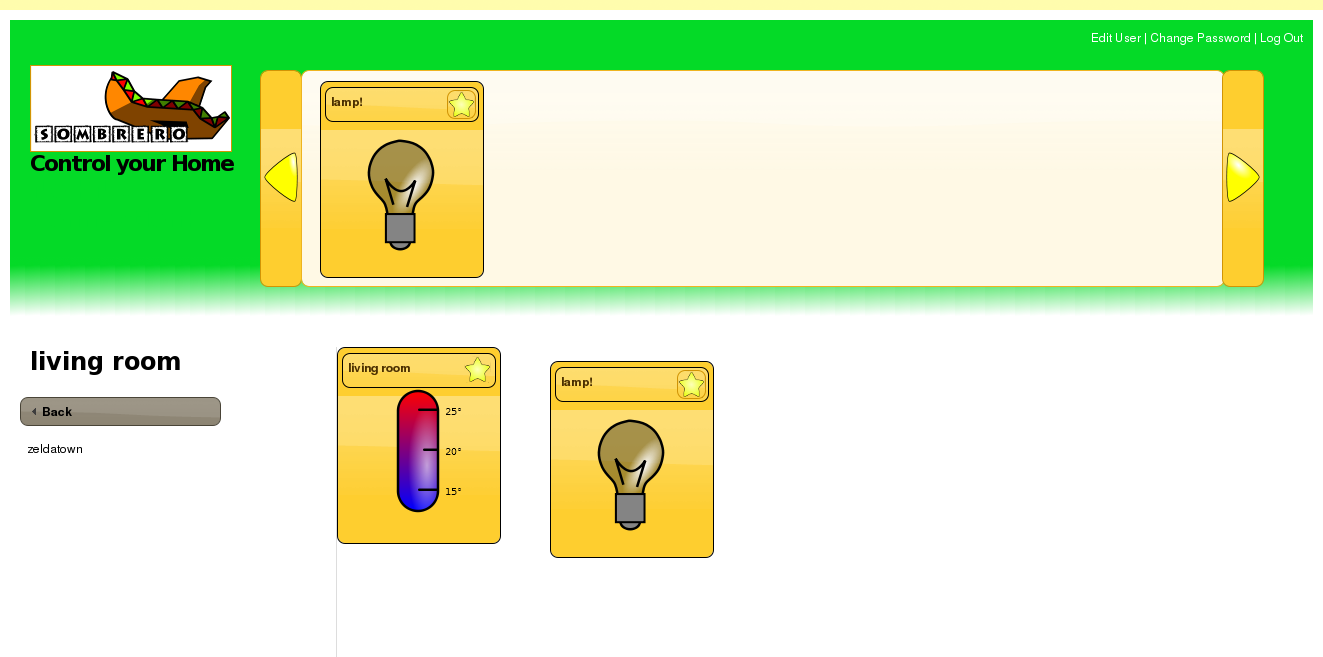
\includegraphics[width=0.80\linewidth]{iteration2.png}
  \caption{shiny new style}
  \label{fig:iterations2}
  \end{figure}

\clearpage
\subsection{Iteration 3 - Finishing}
  As we had little time for the implementation, the third iteration was also the last one. Core functionality was in place, but the whole image was a bit rough around the edges. Widgets still had some bugs and database functionality was mostly hidden behind secret URLs.

  In this iteration we set out to polish the application for shipping and further improve functionality. Unfortunately, Gabriel got sick and we had to drop most of the planned functionality additions. Another goal for this iteration was to clean up the code so it would be easier to read and make additions.

  Gabriel made great improvements to the widgets, fixing lots of bugs and cleaning the code to readability. He also improved widget handling by disallowing them to overlap or leave their predefined space. Another big point of improvement is the separate dialog design he established during this iteration, making dialogs more beautiful and usable.

  Alexander improved user management and widget handling on the server side. He implemented the user list, which allows the administrator to modify other user's accounts. He also wrote a framework which allows widgets to be updated client-side in response to server-side events, which both of us had spent a lot time planning. In adition, Alexander created a grouping system for widgets which was needed for this to work.

  In the end, we managed to get most of our ideas done, creating a complete piece of software. While a bit of further testing couldn't hurt, we believe it is relatively stable, useable and comfortable.

  \begin{figure}[h]
  \centering
  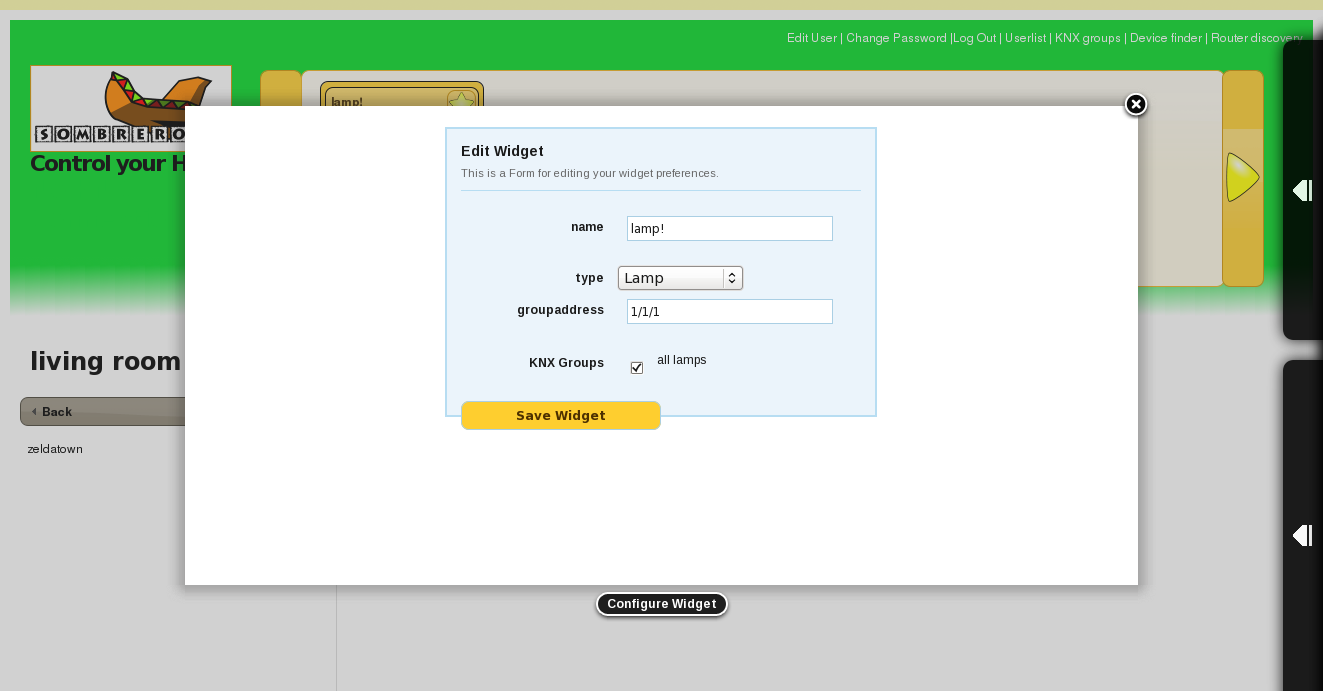
\includegraphics[width=0.80\linewidth]{iteration3f2.png}
  \caption{new dialogs}
  \label{fig:iterations3f1}
  \end{figure}

  \begin{figure}[h]
  \centering
  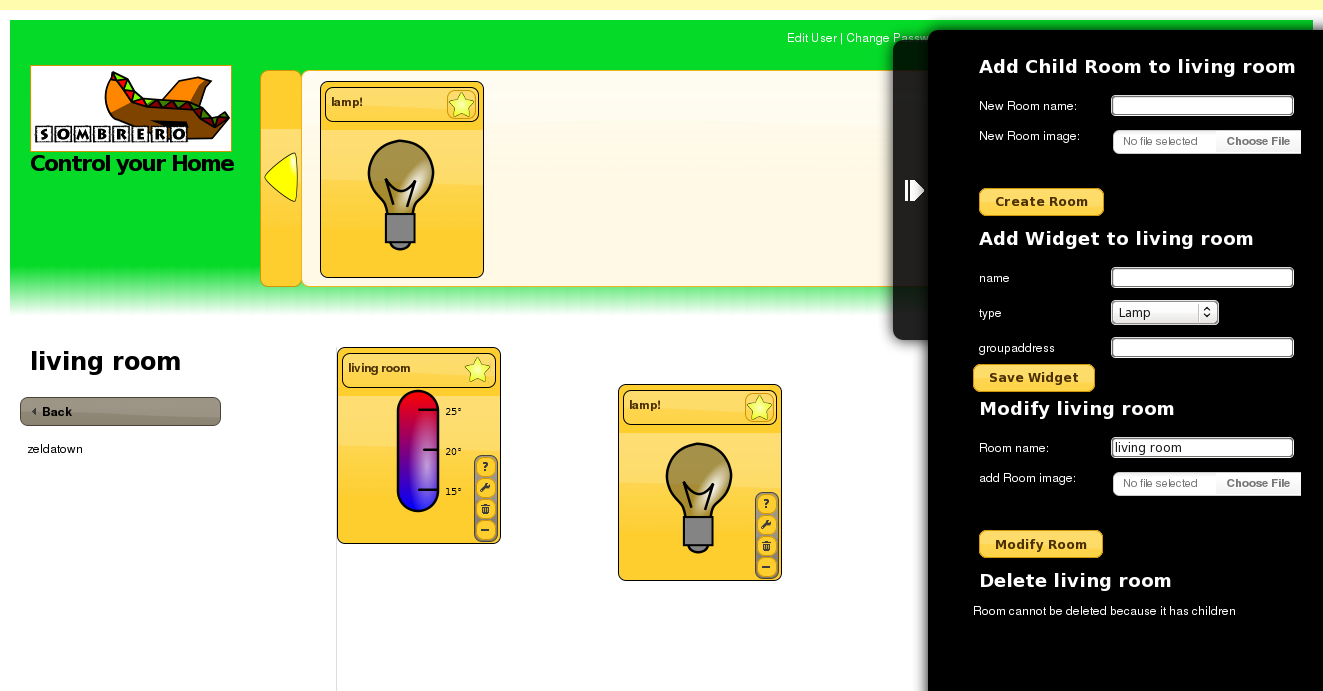
\includegraphics[width=0.80\linewidth]{iteration3f1.png}
  \caption{improved admin mode}
  \label{fig:iterations3f2}
  \end{figure}
